%%%%%%%%%%%%%%%%%%%% author.tex %%%%%%%%%%%%%%%%%%%%%%%%%%%%%%%%%%%
%
% sample root file for your "contribution" to a contributed volume
%
% Use this file as a template for your own input.
%
%%%%%%%%%%%%%%%% Springer %%%%%%%%%%%%%%%%%%%%%%%%%%%%%%%%%%%%%%%%%

\title{Tropical Cyclone - Storm Surge}
% Use \titlerunning{Short Title} for an abbreviated version of
% your contribution title if the original one is too long
\author{
    \textbf{Andrew Kennedy} 
    \and {George Deodatis}
    \and {Ajay Harish}
    \and {Rick Luettich}
    \and {Lance Manuel}}
\tocauthor{}
\authorrunning{Andrew Kennedy et al.}
% Use \authorrunning{Short Title} for an abbreviated version of
% your contribution title if the original one is too long
%\institute{Name of First Author \at Name, Address of Institute, %\email{name@email.address}
%\and Name of Second Author \at Name, Address of Institute %\email{name@email.address}}
%
% Use the package "url.sty" to avoid
% problems with special characters
% used in your e-mail or web address
%
\maketitle

Simulations of coastal storm surge are used for planning, forecasting, nowcasting, hindcasting, climatological studies, and risk evaluation; the need for surge studies has been continual over recent years and there is an ongoing need for trained professionals. The largest surges occur from tropical cyclones, but strong winter storms may also generate high water levels.

Surge studies are in many ways broadly similar: a wind and pressure field forces a hydrodynamic model, potentially inundating areas of interest \citep{njcoast2018implementation}. Details of modeling differ, with numerics, resolution, bottom friction, and theoretical assumptions as noticeable differences. Some systems include additional components such as wave setup and runup, while these are neglected by others. Atmospheric forcing can either be raster-based, where large-scale wind and pressure fields force the modeling system, or may arise from a tropical or extratropical storm scenario described by a storm track and set of parameters describing strength and size. These simulations yield geospatially distributed estimates of storm surge (storm-induced rise in seawater levels, primarily caused by wind) for the purposes of direct and indirect loss assessment for coastal communities \citep{jacob2011responding}. Estimates of storm-induced inundation, due to combined effects of storm surge and waves driving water over land, are important outputs from any simulation environment that help quantify damage to structures as well as above and below ground civil infrastructure.

Because surge models can be expensive, in general there is a need to manage the tradeoff between model fidelity and computational efficiency. One method that has seen increasing adoption in recent years uses surrogate models. Given a database of high-fidelity model runs to be used as a training set, surrogate models can reduce CPU times of model runs from hundreds and even thousands of hours to minutes and enable computationally efficient means to characterize uncertainty in the hazard (e.g., the hurricane track) for the purposes of risk assessment \citep{kijewski-correa2014cybereye}. However, these require large-scale training sets that may not be straightforward to generate. 

\section{Common Modeling Approaches}
\label{sec:storm_surge_methods}

This section examines the three classes of models commonly coupled to capture storm surge and accompanying wave effects nearshore and overland, as well as surrogate models that can be tailored to these coupled models for a computationally efficient simulation alternative. Note: this is not an exhaustive presentation of the simulation tools available for coastal hazards but focuses only on those viewed as the industry standard. 

\subsection{Storm surge heights and inundation}

Numerical models for storm-surge simulations are typically based on single-layer (or sometimes multi-layer) depth averaged shallow water equations describing fluid motion driven by storm winds and pressure. These simplifications are necessary as a full Navier-Stokes based approach is computationally infeasible. The available numerical models differ in their computational solution strategies, with implications for the spatial and temporal resolution of the simulations, the required computational resources and runtimes, and the required input data and model parameters. Generally, these models capture the amplitude of long-period, long-gravity waves and do not simulate short-period wave effects, which are addressed in subsequent sections. Models may be distinguished by resolution, numerics, assumptions, and computational efficiency. Models described here are:

\begin{enumerate}
    \item Sea, Lake and Overland Surges from Hurricanes  (SLOSH)
    \item ADvanced CIRCulation model (ADCIRC)
    \item Delft3D 
    \item Finite Volume COMmunity Model (FVCOM)
    \item GeoClaw
\end{enumerate}

\paragraph{SLOSH} The National Weather Service (NWS) utilizes a storm-surge model called Sea, Lake and Overland Surges from Hurricanes (SLOSH), which solves the shallow water equations using structured curvilinear grids \citep{jelesnianski1992NWS48}. It was developed to provide real-time estimates of storm surge on a single computational core; therefore, the grid resolution and the resulting spatial resolution of the results are fairly coarse. As reported by Mandli and Dawson (2014), a primary limitation of SLOSH is “the limited domain size and extents allowed due to the grid mapping used and formulation of the equations.” Nevertheless, since its initial development, SLOSH has continued to be updated and is used for real-time forecasts of surge for public advisories and to inform emergency responders. SLOSH is very computationally efficient, and this allows it to perform probabilistic simulations of storm surge prior to a hurricane landfall using several thousand runs to obtain some measures of the potential surge if storm tracks and intensities change. Because SLOSH has been used for many years and does not contain all modern features, it may at some point be transitioned to a different model, the most likely being the Coastal and Estuarine Storm Tide model (CEST) \citep{zhang2017transition}. 
% \newline

\paragraph{ADCIRC} The ADvanced CIRCulation (ADCIRC) methodology is commonly regarded as the state-of-the-art in high resolution coastal storm-surge simulation \citep{luettich1992adcirc}, capable of providing significantly more accurate simulations than methods based on SLOSH \citep{resio2008modeling} in near-shore coastal regions. As such, ADCIRC is the preferred methodology for coastal storm-surge investigations by the U.S. Army Corps of Engineers (USACE) and is one of the two models certified for the generation of FEMA Digital Flood Insurance Rate Maps (DFIRMSs). ADCIRC solves the depth-averaged shallow water equations describing on a rotating earth, formulated using the traditional hydrostatic pressure and Boussinesq approximations, and discretized in space using the finite-element method and in time using the finite-difference method. ADCIRC can be run either as a 2D depth integrated (2DDI) model or as a 3D model, with elevation resulting from the solution of the depth-integrated continuity equation in generalized wave-continuity equation (GWCE) form. Furthermore, velocity is obtained from the solution of either the 2DDI or 3D momentum equations, retaining all nonlinear terms. ADCIRC simulations have been validated for major hurricanes such as Katrina, Ike, Gustav, and Iniki \citep{kennedy2011origin,kennedy2012tropical}. ADCIRC has been parallelized efficiently, with linear speedups to hundreds or thousands of cores for large domains. 
% \newline

\paragraph{Delft3D} Delft3D-Flow is the second model certified for FEMA DFIRM generation. It is based on shallow water equations in either depth-averaged or multi-layer formulation, and is used widely among engineering consultants and researchers \citep{hu2015numerical,vousdoukas2016projections}. Delft3D may be run in either serial or parallel modes, with typical parallel runs using tens of cores. The Delft3D-Flow surge model is a part of a larger suite of interrelated models that include spectral wave, and coastal runup/morphological evolution \cite{deltaressystems2011delft3d}. 
% \newline

\paragraph{FVCOM} FVCOM is s finite volume-based model that has been used by numerous academic researchers to study storm surge \citep{kerr2013ioos,rego2010storm}. It is based on unstructured meshes, and shows similar skill to other models when run on a similar grid. The use of FVCOM for storm surge studies is in some ways a simplification of the full model, which includes momentum, continuity, temperature, salinity and density. It was originally developed for coastal and estuarine circulation by the oceanographical community, and is fully open source \citep{chen2003unstructured}. 
% \newline

\paragraph{GEOCLAW} GEOCLAW, the final computational platform, lies between SLOSH and ADCIRC in terms of modeling resolution and computational cost. Originally developed to simulate tsunami inundation, GEOCLAW has recently been adapted to simulate storm surge \citep{berger2011geoclaw, Mandli et al., 2014}. Based on the CLAWPACK software libraries \citep{leveque2002finite}, GEOCLAW is an open-source, finite-volume, wave-propagation numerical model used to estimate hurricane-induced storm surge along a coastline. For overland flooding, the model uses Manning's n to parameterize roughness due to objects such as trees and small-scale structures that cannot be resolved computationally. Adaptive mesh refinement allows GEOCLAW to place computational resources where and when they are needed during a simulation. Thus, the overall cost of the simulation is reduced, while retaining the same or similar accuracy characteristics to ADCIRC. Shown in Figure \ref{fig:GEOCLAW_ADCIRC_comparison} is a comparison of results calculated using GEOCLAW versus ADCIRC. 

\begin{figure}[htb]
    \centering
    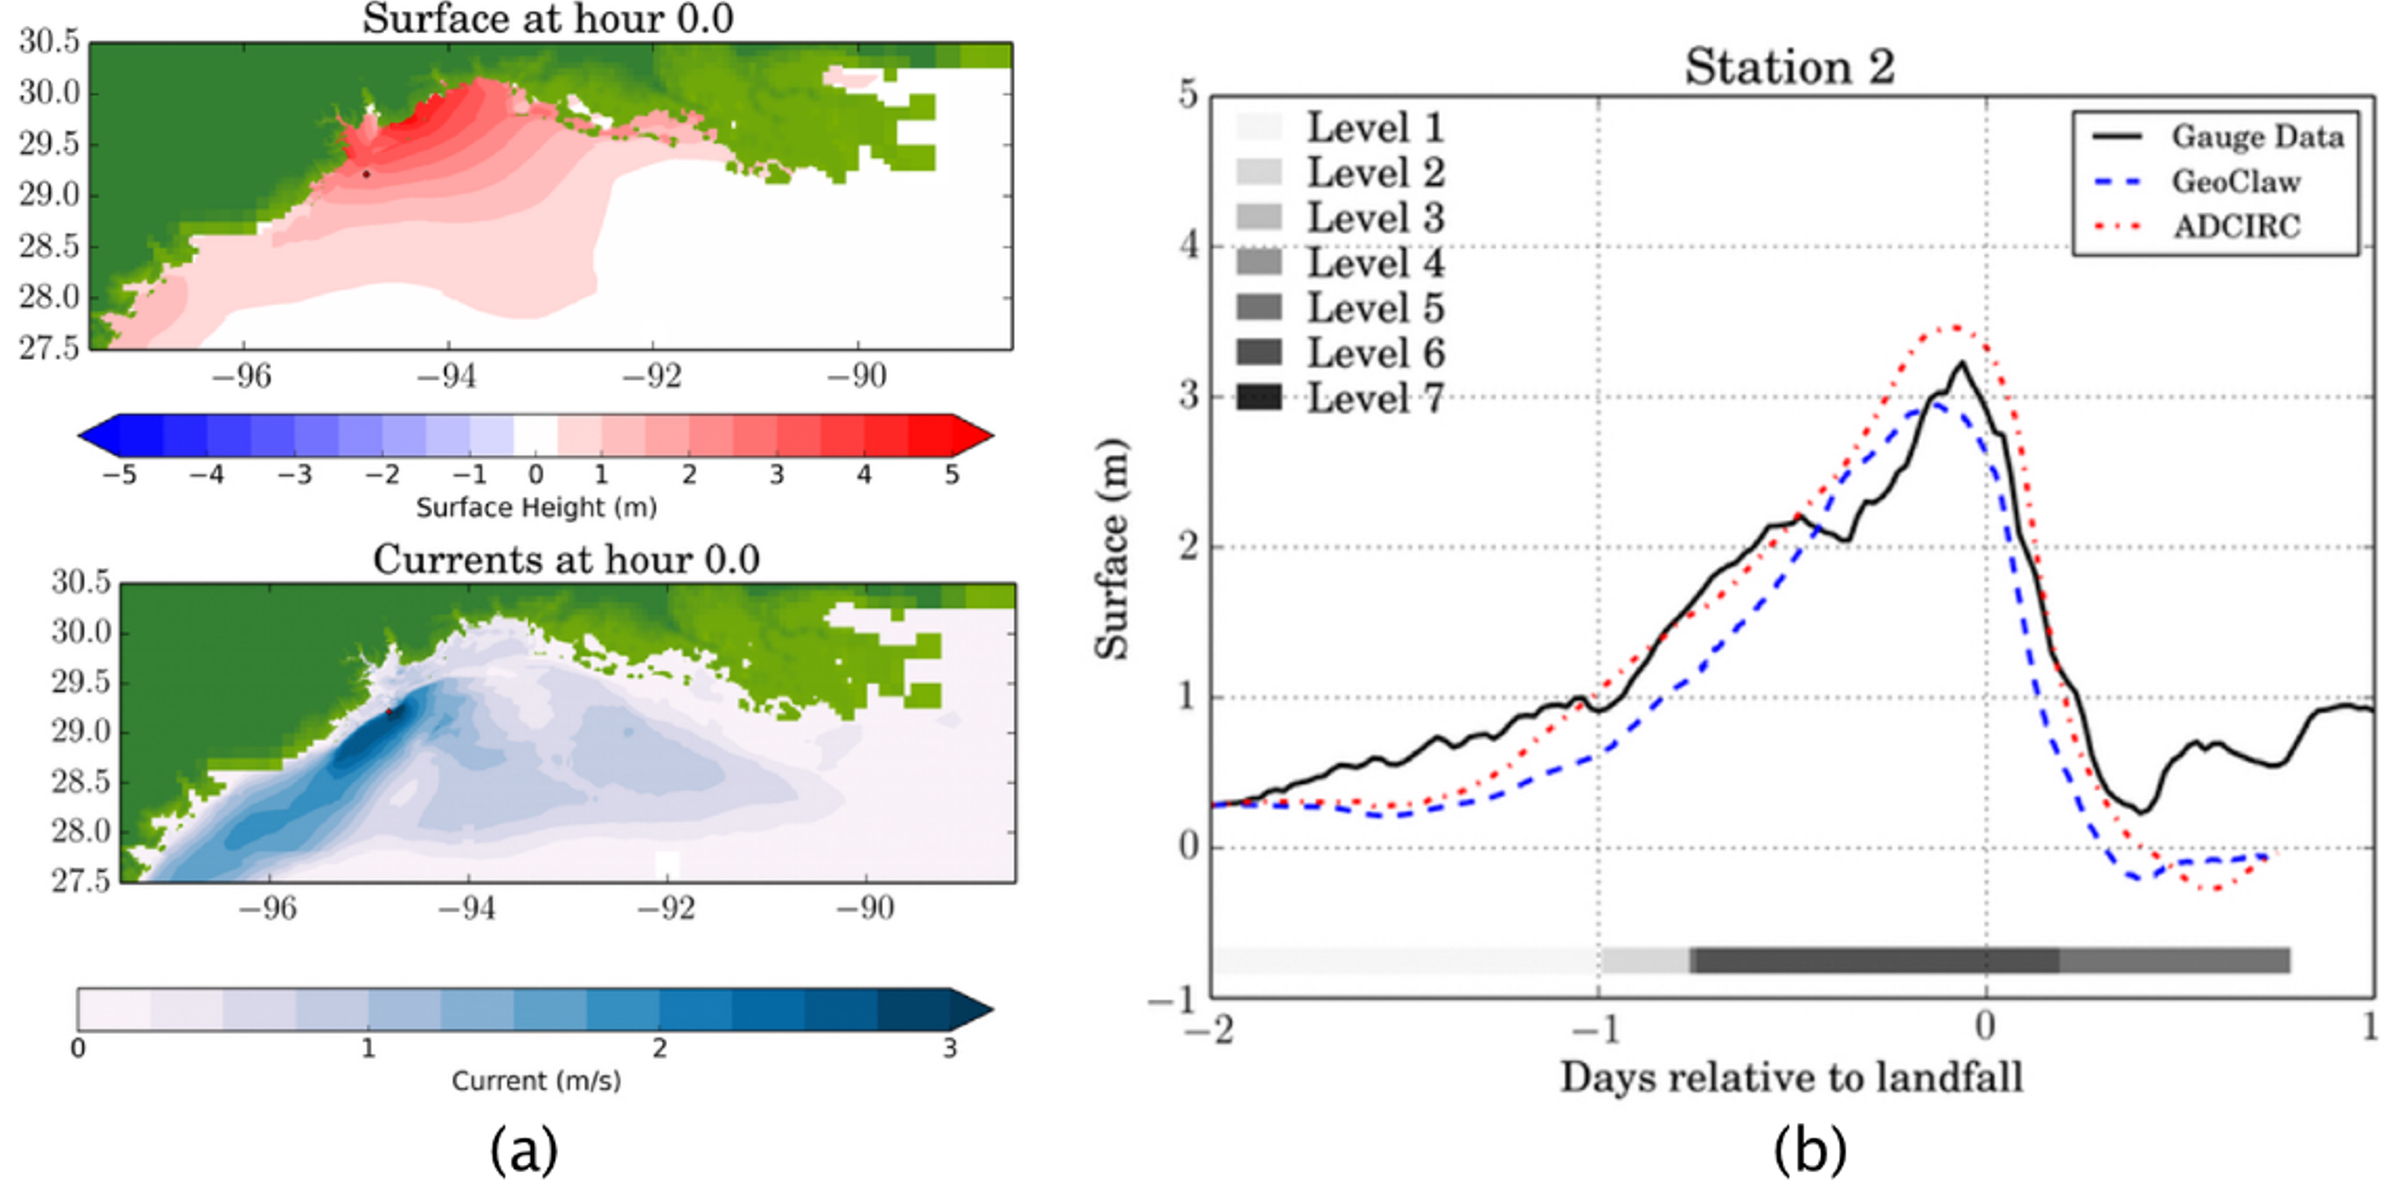
\includegraphics[width=1.0\textwidth, angle = 0]{Figures/GEOCLAW_ADCIRC_comparison.png}
    \caption{(a) A snapshot of a GEOCLAW storm surge simulation of Hurricane Ike at landfall; and (b) tide gauge data computed from GEOCLAW and ADCIRC along with observed data at the same location. \citep{mandli2016clawpack}}
    \label{fig:GEOCLAW_ADCIRC_comparison}
\end{figure}

\subsection{Spectral wave models}

The platforms described above simulate slowly-varying surge heights but do not capture local wave effects. To do this, requires a separate wave model, either run as a fully-coupled system where both models pass information to each other, or as a one-way loosely coupled system. In two-way coupling, wave models pass radiation stresses to the surge model, while the surge model passes water levels and currents to the wave model. In one-way coupling, which is less accurate, the wave model is run at some given water level and radiation stresses are passed to the surge model.

The most common model used is Simulating WAves Nearshore (SWAN), which solves equations for wave spectral density in both frequency and direction \citep{zijlema2010computation}. ADCIRC has been coupled previously with SWAN \citep{dietrich2011modeling,kennedy2012tropical}. The most recent North Atlantic Coastal Comprehensive Study (NACCS) \citep{usace2015north} employs STWAVE, which is a steady-state, finite difference spectral model for nearshore wind-wave growth and propagation based on the wave action balance equation \citep{smith2001stwave}. STWAVE simulates depth-induced wave refraction and shoaling, current-induced refraction and shoaling, depth- and steepness-induced wave breaking, diffraction, wave growth because of wind input, and wave–wave interaction and white capping that redistributes and dissipates energy in a growing wave field. Figure \ref{fig:surge_validation} validates the coupled hydrodynamic models used in the NACCS by comparing to measurements across historical storms or tide predictions \citep{nadal-caraballo2015north}. Additional wave models in use include WaveWatch III \citep{smith2018validation}, which is also NOAA’s operational forecast model. 

\begin{figure}[htb]
    \centering
    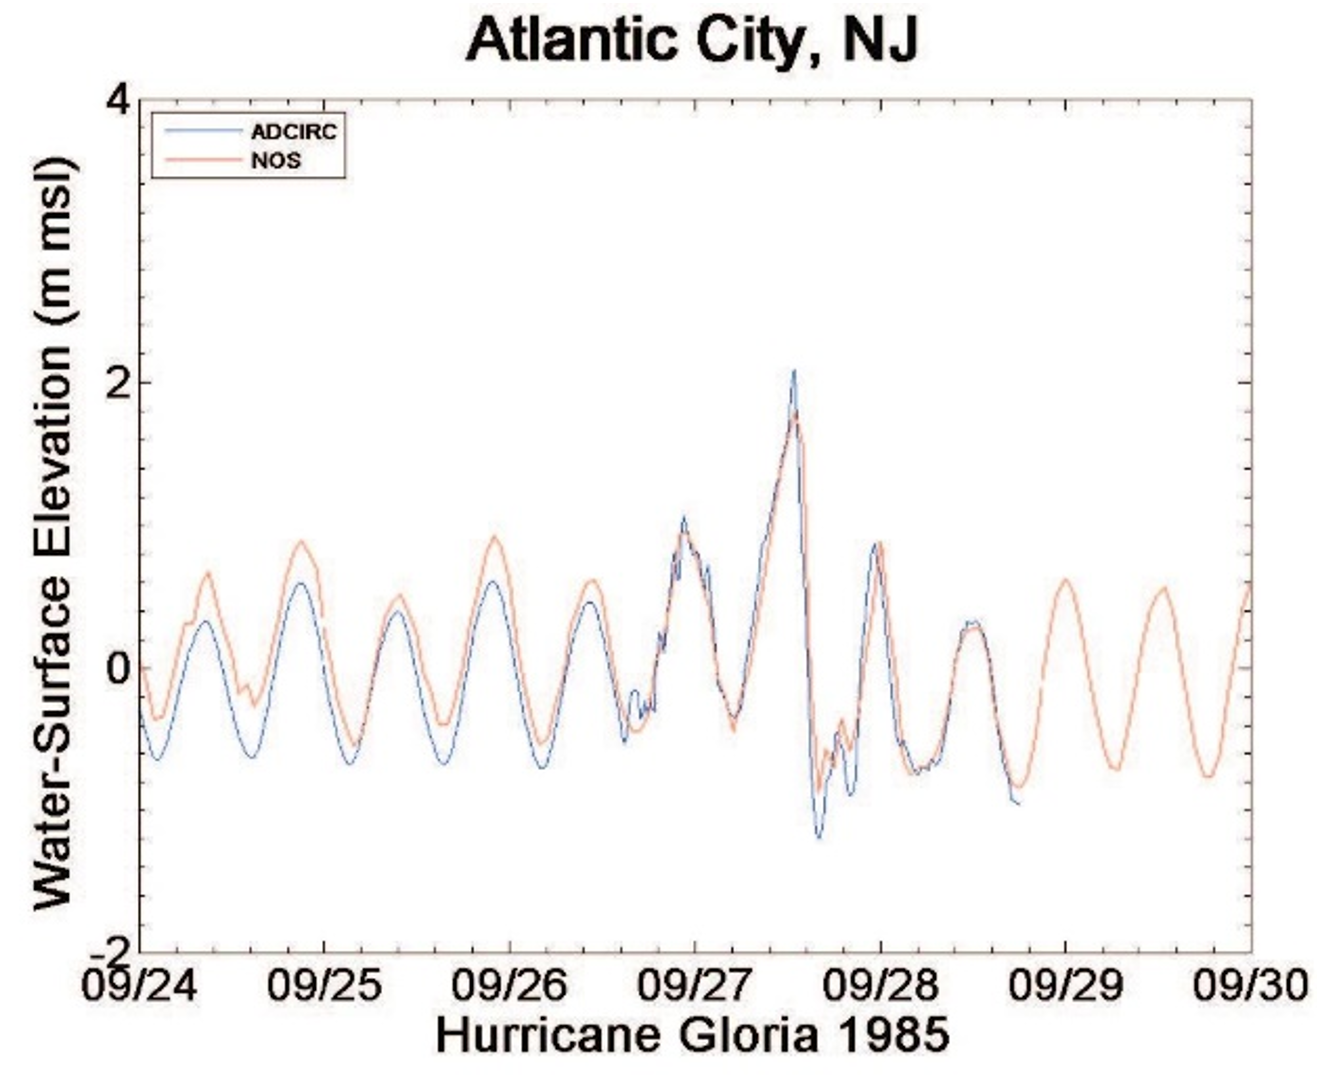
\includegraphics[width=0.5\textwidth, angle = 0]{Figures/surge_validation.png}
    \caption{Validation of surge simulation in Atlantic City using coupled ADCIRC-STWAVE for historical storm Hurricane Gloria, courtesy of USACE \citep{nadal-caraballo2015north}}
    \label{fig:surge_validation}
\end{figure}

\subsection{Wave run up overland}

Even when coupled with an appropriate nearshore wave model, surge models simulate only the storm-surge elevation and not the additional impact of wave run up, which is particularly important for predicting losses to buildings and infrastructure in a storm event. Supplementary wave run-up simulations are required to capture the interaction of the waves with the shoreline and any coastal protective features along coastal transects. Two types of models are common:

\begin{enumerate}
    \item Wave-Group Envelope models, where the effects of unsteady wave groups on long-wave surge and runup drive time-varying water levels in the nearshore and at the moving shoreline. However, these models do not model individual wave runup, which can be important in certain instances. By far the most common model of this type is XBeach \citep{roelvink2009modelling}, which is also commonly used to estimate morphological evolution over short time periods. Models of this type require O(10m) resolution to resolve important processes, and thus have much heavier computational requirements than both spectral wave and surge models for a similar domain. Thus, they are generally limited to km-to-tens of km-scales for simulations. 
    \item Wave-resolving models, where individual points on the water surface are defined to model the evolution of the detailed wave shape over arbitrary bathymetry. The most common models of this type use different versions of Boussinesq models \citep{lynett2002modeling,kennedy2000boussinesq,nwogu2010infragravity}, which are derived from Taylor series expansions about the long wave limit. Wave-resolving models can simulate both wave group runup and runup from individual waves, but may require resolution of O(5m) or finer in the nearshore. Although these models may be used to simulate nearshore behavior of entire storms, they are quite computationally expensive (far more so than wave-group envelope models), and often one-dimensional transects are chosen for representative simulations. Transect locations are generally selected by segmenting the defined coastline in the areas of interest and selecting the transect density proportional to computational demand. Each transect is then discretized to capture the site-specific bathymetry (offshore) and topography (onshore) along its length. Moreover, transects must accurately capture the current condition of coastal protective features, e.g., dunes, in order to effectively predict the total run up inland. Inputs from the surge and spectral wave models are fed into a one-dimensional (1D) Boussinesq model executed at the pre-selected transects in order to estimate the wave run up overland \citep{demirbilek2009wave}. 
\end{enumerate}

\subsection{Surrogate modeling approach}

Given the high degree of sophistication and computational resources required to execute just one high-fidelity simulation (e.g., an ADCIRC+STWAVE/SWAN run), alternative simulation tools have been developed recently to enable a wider range of users to employ these models for hazard characterization, risk assessment, and design of coastal protective strategies. Most notably, surrogate modeling approaches can efficiently evaluate hurricane wave and surge responses by leveraging databases of existing high-fidelity simulations normally driven by a collection of historical and synthetic hurricane tracks \citep{usace2015north}. This is made possible by formulating a simplified description of a storm scenario by a small number of model parameters corresponding to its characteristics at landfall. The scenarios in the database are then parameterized with respect to this model parameter vector and ultimately provide an input–output dataset. Because the geospatial representation often covers a regional coastline (typically represented by a large number of nodes) and resolves the coastal hazards at different times during the hurricane’s history, the dataset is often high-dimensional. After correcting for any dry nodes at inland locations, the surrogate model is then built to approximate this input-output relationship. 

Although the initial implementations of the surrogate modeling approach relied upon a moving least-squares-response surface methodology, more recent implementations for natural hazard risk assessment now employ a Kriging metamodel for this purpose \citep{jia2013kriging}. To further reduce the computational burden pertaining to both speed of execution and more importantly memory requirements, this approach is coupled with principal component analysis (PCA) as a dimensional reduction technique. The metamodel is then developed in this low-dimensional latent space (in this case below 100), with the predictions transformed back to the original space for visualization purposes. This PCA implementation contributes to very large computational savings necessary to enable the evaluation of a large ensemble of scenarios as required for a probabilistic evaluation while circumventing the need for HPC resources \citep{jia2013kriging}. Validation of these surrogate models using leave-one-out cross validation \citep{taflanidis2017advances} suggested high accuracy, with coefficient of determination close to 0.96 and a correlation coefficient close to 98\%. By permitting rapid evaluation of alternate storm scenarios, surrogate models offer an effective way to communicate simulation results to urban planners and emergency managers. One such implementation is a software system developed to assess storm surge risks on the coast of New Jersey \citep{njcoast2018implementation}.

\section{Required Inputs and Resulting Outputs}
\label{sec:storm_surge_io}

High-fidelity computational simulations of coastal hazards require: (1) storm track information, including the relevant description of the hurricane wind and pressure fields to drive the model; (2) the topography and bathymetry along the coastline; and (3) the land use/land cover data for the simulation of wave run up on shore. The simulations are inherently sensitive to assumptions made regarding tides at the time of landfall. The coupling of a storm surge + nearshore wave + wave run-up model will yield geospatially-distributed, time-dependent responses, i.e., the mean water elevation, max water elevation, max water depth, and significant wave height (or limit of moderate wave action). Such responses can be generated either by the coupling of the aforementioned high-fidelity models or a surrogate model tuned to a database of results from these models. A brief summary of specific inputs required for storm surge models, the wave run-up models, and the related surrogate models are as follows:
% \newline

\paragraph{Storm Surge Models} All storm surge models require variations of the same inputs, potentially in much different forms. All models require:

\begin{itemize}
    \item Spatial and temporal information about wind fields and pressure. This may be in the form of gridded data, or in the form of parameterized wind and pressure fields,
    \item Bathymetry and topography over the entire domain,
    \item Frictional information, whether in the form of direct frictional coefficients or roughness, or land use/land cover information that is converted to frictional resistance. 
    \item Boundary conditions at the domain limits
\end{itemize}

\noindent
Many models will also require:

\begin{itemize}
    \item Information on tidal forcing when real dates are being simulated
    \item Computational settings, particularly for parallel systems
\end{itemize}

\paragraph{Wave Run-up Models} In addition to the topography and bathymetry data at each identified transect, and potentially frictional information, the wave run-up model must receive wave and water level inputs from the coupled wave-storm surge model.
% \newline

\paragraph{Surrogate Models} Inputs to the surrogate model are twofold: the primary input required to develop the surrogate model itself is the aforementioned database of high-fidelity simulations for a family of storm tracks that may include tropical and extra-tropical storms. Once developed, users of the surrogate model input only a collection of parameters necessary to describe the storm scenario based on its characteristics at landfall: 

\begin{enumerate}
    \item reference location (latitude, longitude)
    \item track heading (angle)
    \item central pressure (or pressure difference)
    \item forward speed
    \item radius of maximum winds
\end{enumerate}

More recently, this implementation was further simplified to enable simulation based on only reference location and storm strength (Category 1-5) \citep{njcoast2018implementation}. It is important to emphasize that once the surrogate model is tuned to high-fidelity simulation data for a specific geographic location, it can efficiently provide predictions for storm scenarios of varying characteristics, even if that scenario does not match any of those within the original database of high-fidelity simulations. 

\section{Primary Software Environments}
\label{sec:storm_surge_tools}

The execution environments are briefly summarized below, but only for models included in the NHERI DesignSafe suite. 
% \newline

\paragraph{ADCIRC and coupled models} ADCIRC has been optimized by unrolling loops for enhanced performance on multiple computer architectures and can be executed on any operating system with a working FORTRAN compiler. These include large commercial Unix systems (IBM Power \& Blue Gene, Cray, SGI, and Sun), Linux- and FreeBSD-based clusters, and personal workstations running Windows or Mac OSX. ADCIRC includes MPI library calls to allow it to operate at high efficiency on parallel computer architectures, which is often preferable for simulations over large domains where a single hurricane realization can require thousands of CPU hours. Coupled ADCIRC+SWAN models are available on all of the aforementioned platforms (with the exception of Windows), while the coupled ADCIRC+STWAVE model is available on all the platforms including Windows PCs as part of the Coastal Storm Modeling System (CSTORM-MS). ADCIRC and its parallel implementation, PADCIRC, along with the coupled ADCIRC+SWAN software, are available on DesignSafe.
% \newline

\paragraph{CLAWPACK/GEOCLAW} Clawpack (``Conservation Laws Package'') is a collection of finite-volume methods for linear and nonlinear hyperbolic systems of conservation laws. Clawpack employs high-resolution Godunov-type methods with limiters in a general framework applicable to many kinds of waves. GEOCLAW is an open-source, finite-volume, wave-propagation software, which is implemented in CLAWPACK, to estimate hurricane-induced storm surge with adaptive mesh refinement. The CLAWPACK 5.4.0 suite and the GEOCLAW tools are available through DesignSafe.
% \newline

\paragraph{SLOSH} SLOSH (Sea, Lake and Overland Surges from Hurricanes) is a computerized numerical model developed by the National Weather Service (NWS) to estimate storm-surge heights determined from historical, hypothetical, or predicted hurricanes by taking into account the atmospheric pressure, size, forward speed, and track data. These parameters are used to create a model of the wind field that drives the storm surge. The SLOSH model consists of a set of physics equations that are applied to a specific locale's shoreline to incorporate the unique bay and river configurations, water depths, bridges, roads, levees, and other physical features. Storm-surge forecasts developed using SLOSH are available at https://www.nhc.noaa.gov/surge/slosh.php.

\section{Major Research Gaps}
\label{sec:storm_surge_gaps}

Although many research topics remain, the major issue remaining with storm surge models is that the fast models are less accurate, and the accurate models are slow. Thus, it remains impossible to run the most accurate models for the hundreds or thousands of simulations required to obtain surge probabilities prior to a landfalling hurricane, or to simulate very long climatological records. Three methodologies hold the potential to improve the accuracy/speed tradeoff:

\begin{itemize}
    \item Surrogate or reduced models that make use of previous high fidelity model runs to develop simpler and faster models for new cases. This was discussed earlier; AI also falls into this broad category,
    \item Improved computational schemes that improve parallel performance for slower models, or improve accuracy for faster models,
    \item Improved theoretical schemes to increase the accuracy on coarse grids. The subgrid model corrections fall into this category, and have been shown to increase accuracy greatly \citep{kennedy2019subgrid}.
\end{itemize}

The next major research gap is very difficult but extremely important: large scale surge models do not account for morphological evolution during storms. Dune or beach erosion, and levee failure, are two examples of morphological feedbacks that may affect significantly surge inundation, and estimates of post-storm erosion are also greatly desired. This has been a long-term goal with little progress.

Finally, whether employing these high-fidelity models or a companion surrogate model, the resulting time-evolving water depth and velocity must translate into loadings on buildings and infrastructure. In this regard, these models face similar limitations as wind-field models given the complexity of interactions with their surroundings. Accurately capturing the physics of the flow overland and the effect of its interaction with the built environment on the load description remains a challenging problem, even without further accounting for the effects of debris transported in the flow. Identifying means to reasonably determine the impact of these interactions on the load description—without having to support an intensive CFD investigation—will enable a wider range of researchers to evaluate the impacts of coastal hazards. 
 
% \section{References}
